%%%%%%%%%%%%%%%%%%%%%%%%%%%%%%%%%%%%%%%%%
% Beamer Presentation
% LaTeX Template
% Version 1.0 (10/11/12)
%
% This template has been downloaded from:
% http://www.LaTeXTemplates.com
%
% License:
% CC BY-NC-SA 3.0 (http://creativecommons.org/licenses/by-nc-sa/3.0/)
%
%%%%%%%%%%%%%%%%%%%%%%%%%%%%%%%%%%%%%%%%%

%----------------------------------------------------------------------------------------
%	PACKAGES AND THEMES
%----------------------------------------------------------------------------------------

\documentclass{beamer}
\mode<presentation> {
\usetheme{Madrid}
}
\usepackage{url}
\usepackage{lmodern}
\usepackage{graphicx}
\usepackage{booktabs}

% for mathematics
\usepackage{amsmath}
\usepackage{amsthm}

%----------------------------------------------------------------------------------------
%	TITLE PAGE
%----------------------------------------------------------------------------------------

\title[Financial mathematics with Python]{UROPS Project Presentation 5} % The short title appears at the bottom of every slide, the full title is only on the title page

\author{Wang Zexin} % Your name
\institute[NUS]
{
Chapter 16 Simulation of Financial models\\
of Python for Finance\\[3mm]
\medskip
\textit{Quantitative Finance\\
National University of Singapore\\}
}
\date{\today}

\begin{document}
%----------------------------------------------------------------------------------------
%	TITLE PAGE
%----------------------------------------------------------------------------------------
\begin{frame}
\titlepage
\end{frame}

%----------------------------------------------------------------------------------------
%	TABLE OF CONTENTS
%----------------------------------------------------------------------------------------

%------------------------------------------------
\begin{frame}
\frametitle{Today's Agenda}
\tableofcontents
\end{frame}

%------------------------------------------------
\begin{frame}
\frametitle{Changes due to different Python version}
We are using Python 3.6 while the version in the book is Python 2.7\\
So here is a list of items to change\\[2mm]
\begin{itemize}
	\item print x now becomes print(x)
	\item dict.iteritems() now becomes dict.items()
	\item xrange now becomes range
	\item lambda (k, v) : (v, k) is no longer available
	\item instead we can only use: lambda x : (x[1], x[0])
	\item x / 2 is float division, while x // 2 is integer division
\end{itemize}
\end{frame}

%------------------------------------------------
\section{Simulation of Financial models}

%------------------------------------------------
\begin{frame}
\frametitle{Simulation of Financial models}
\begin{itemize}
	\item Random number generation\\[3mm]
	\item Generic simulation class\\[3mm]
	\item Geometric Brownian motion\\[3mm]
	\item Jump diffusion\\[3mm]
	\item Square-root diffusion\\[3mm]
	\item Wrapper class
\end{itemize}
\end{frame}

\subsection{Random number generation}

%------------------------------------------------
\begin{frame}
\frametitle{Generate standard normally distributed random numbers}
\begin{figure}[H]
	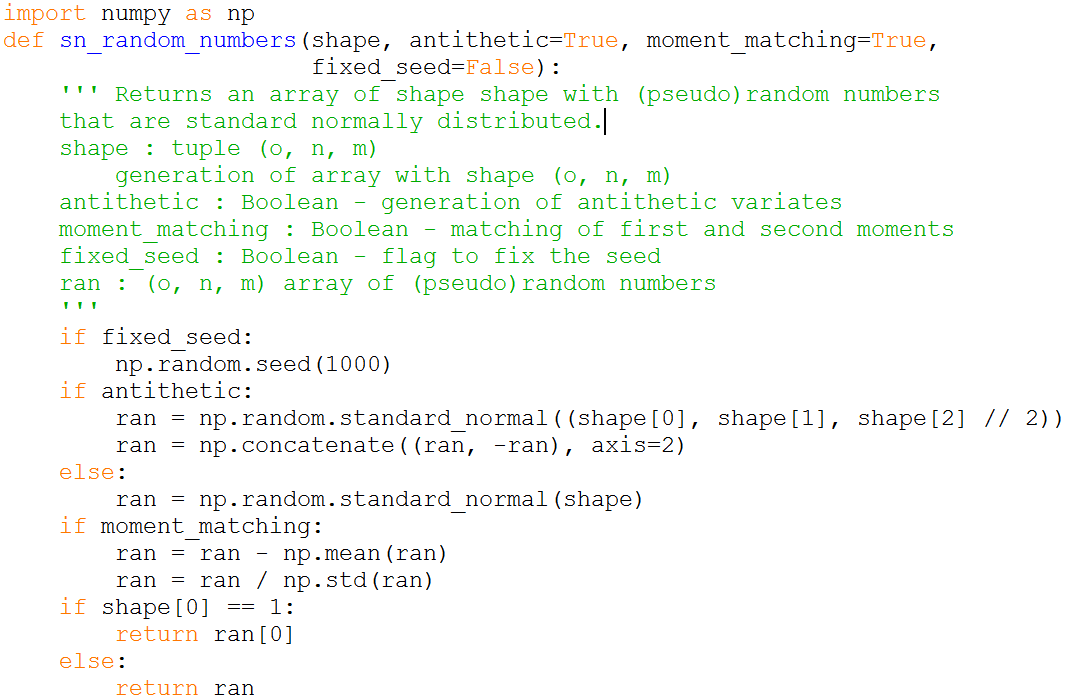
\includegraphics[scale=0.42]{sn_random_numbers.png}
\end{figure}
\end{frame}

\subsection{Generic financial model simulation class}

%------------------------------------------------
\begin{frame}
\frametitle{Generic financial model simulation class}
Below are all the parameters initiated for this class.
\begin{figure}[H]
	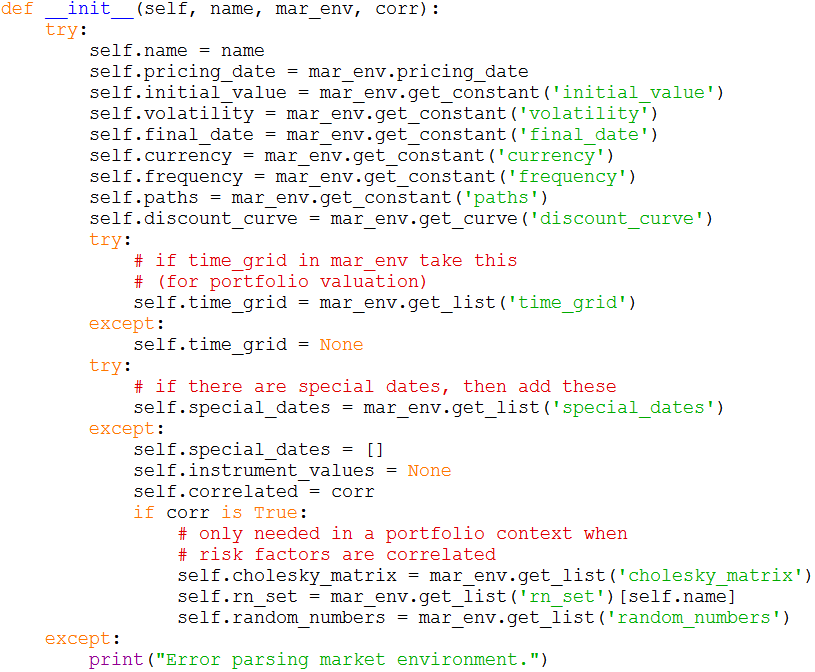
\includegraphics[scale=0.41]{parameters_simulation_class.png}
\end{figure}
\end{frame}

%------------------------------------------------
\begin{frame}
\frametitle{Generic simulation class - generate time grid}
\begin{figure}[H]
	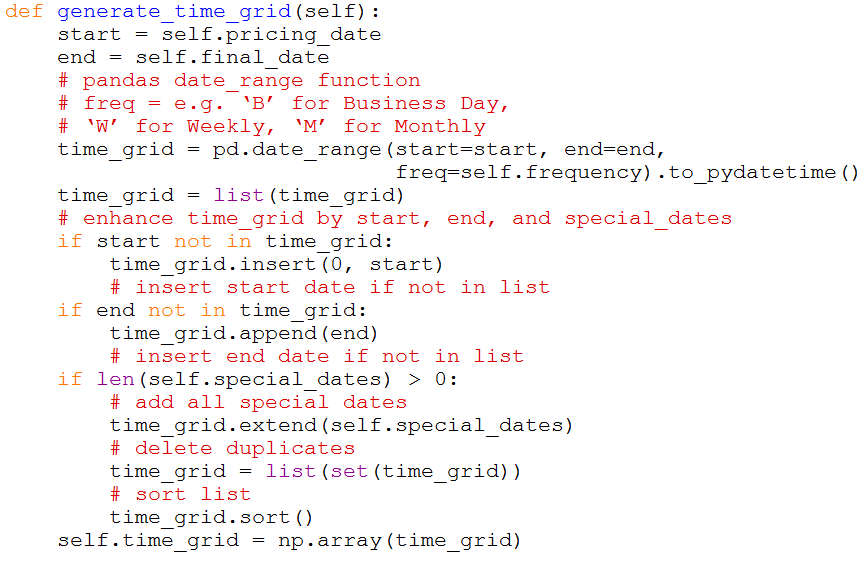
\includegraphics[scale=0.5]{rest_simulation_class_1.png}
\end{figure}
\end{frame}

%------------------------------------------------
\begin{frame}
\frametitle{Generic financial model simulation class}
This method returns the values of instruments built-in.
\begin{figure}[H]
	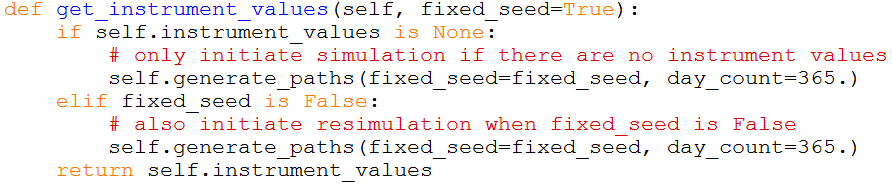
\includegraphics[scale=0.5]{rest_simulation_class_2.png}
\end{figure}
\end{frame}

\subsection{Geometric Brownian Motion}
%------------------------------------------------
\begin{frame}
\frametitle{Geometric Brownian Motion}
$$S_{T} = S_{0}\exp\{(r-\frac{1}{2}\sigma^{2})T + \sigma\sqrt{T}z\}$$
$$S_{t} = S_{t-^{\Delta}t}\exp\{(r-\frac{1}{2}\sigma^{2})^{\Delta}t + \sigma\sqrt{^{\Delta}t}z_{t}\}$$
\end{frame}

%------------------------------------------------
\begin{frame}
\frametitle{Geometric Brownian Motion - implementation}
\begin{figure}[H]
	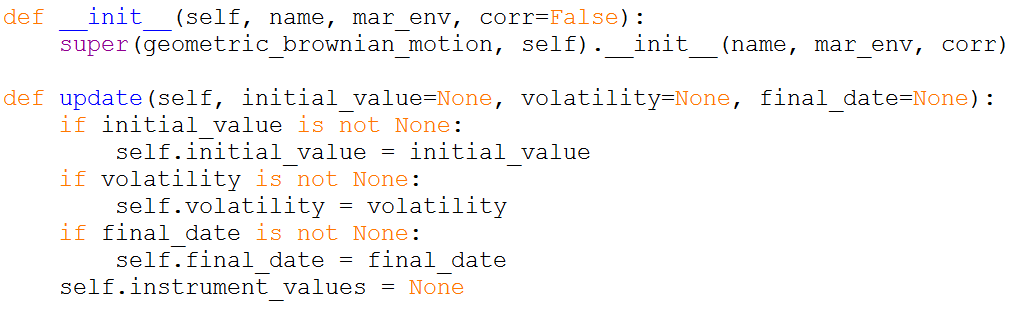
\includegraphics[scale=0.45]{gbm_init_update.png}
\end{figure}
\end{frame}

%------------------------------------------------
\begin{frame}
\frametitle{Geometric Brownian Motion - implementation}
\begin{figure}[H]
	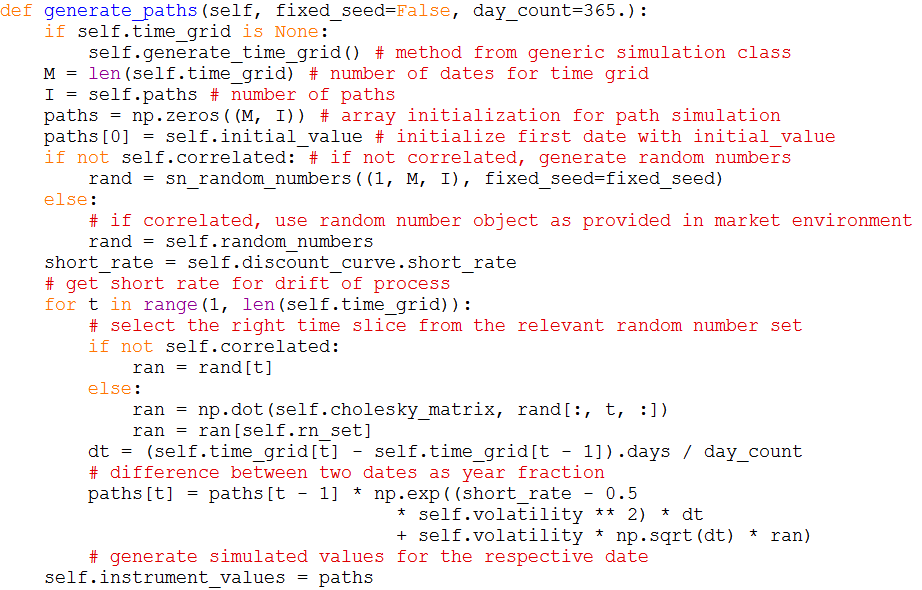
\includegraphics[scale=0.47]{gbm_generate_path.png}
\end{figure}
\end{frame}

%------------------------------------------------
\begin{frame}
\frametitle{Geometric Brownian Motion - Use Case}
\begin{figure}[H]
	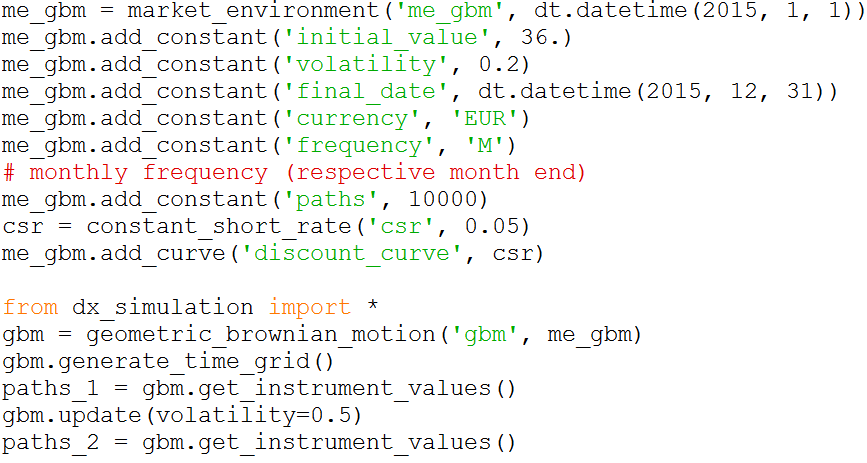
\includegraphics[scale=0.45]{gbm_use_case.png}
\end{figure}
The GBM simulation class is able to:
\begin{itemize}
	\item Import parameters from market environment class
	\item Generate datetime object time grid
	\item Get instrument values based on parameters
\end{itemize}
\end{frame}

\subsection{Jump Diffusion}
%------------------------------------------------
\begin{frame}
\frametitle{Jump Diffusion Model}
\begin{center}
$dS_{t} = (r-r_{\mathrm{J}})S_{t}dt + S_{t}dZ_{t}	+ {\mathrm{J}}_{t}S_{t}dN_{t}$\\[10mm]
	Euler discretization:\\[6mm]
	$S_{t} = S_{t-{^{\Delta}t}} [e^{(r-r_{\mathrm{J}}-\sigma^{2}/2){^{\Delta}t}+\sigma \sqrt{^{\Delta}t}z_{t}^{1}}+(e^{\mu_{\mathrm{J}}+\delta z_{t}^{2}}-1)y_{t}] $
\end{center}
\end{frame}

%------------------------------------------------
\begin{frame}
\frametitle{Jump Diffusion - implementation}
\begin{figure}[H]
	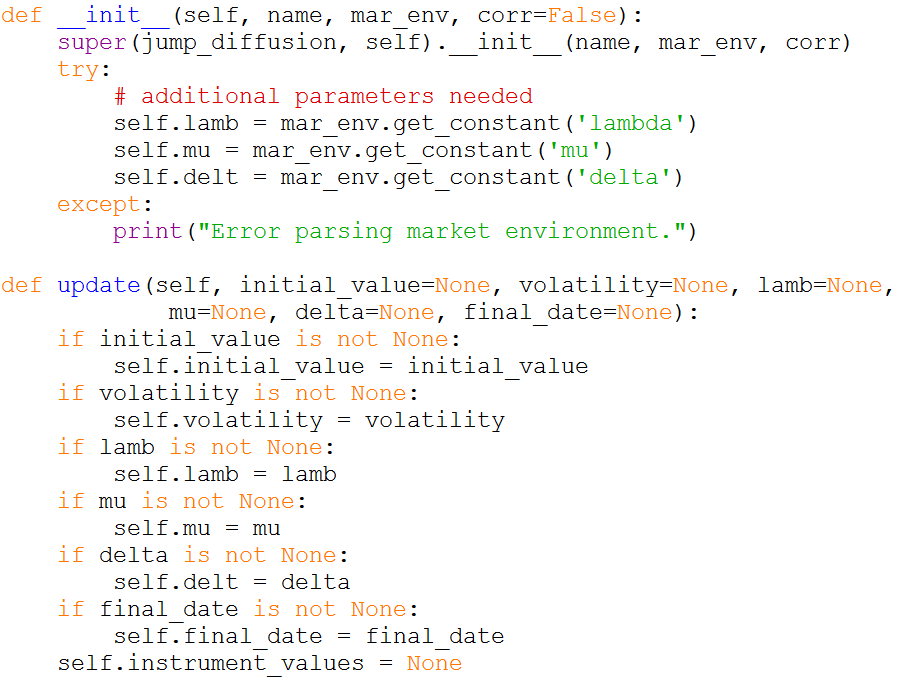
\includegraphics[scale=0.42]{jd_init_update.png}
\end{figure}
\end{frame}

%------------------------------------------------
\begin{frame}
\frametitle{Jump Diffusion - implementation}
This part of generate\_path is repeated, maybe we can capture this feature
\begin{figure}[H]
	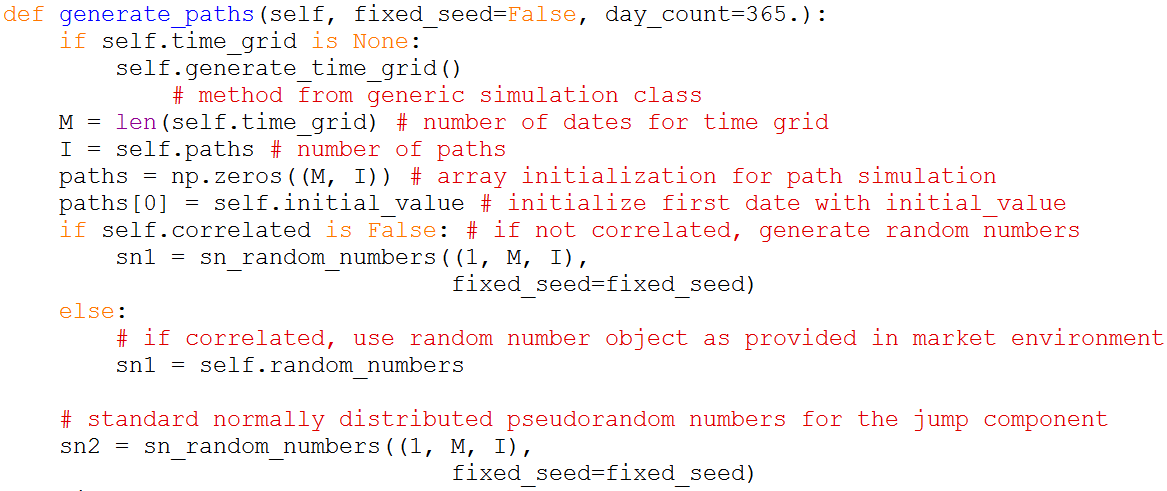
\includegraphics[scale=0.4]{jd_generate_path_1.png}
\end{figure}
\end{frame}

%------------------------------------------------
\begin{frame}
\frametitle{Jump Diffusion - implementation}
\begin{figure}[H]
	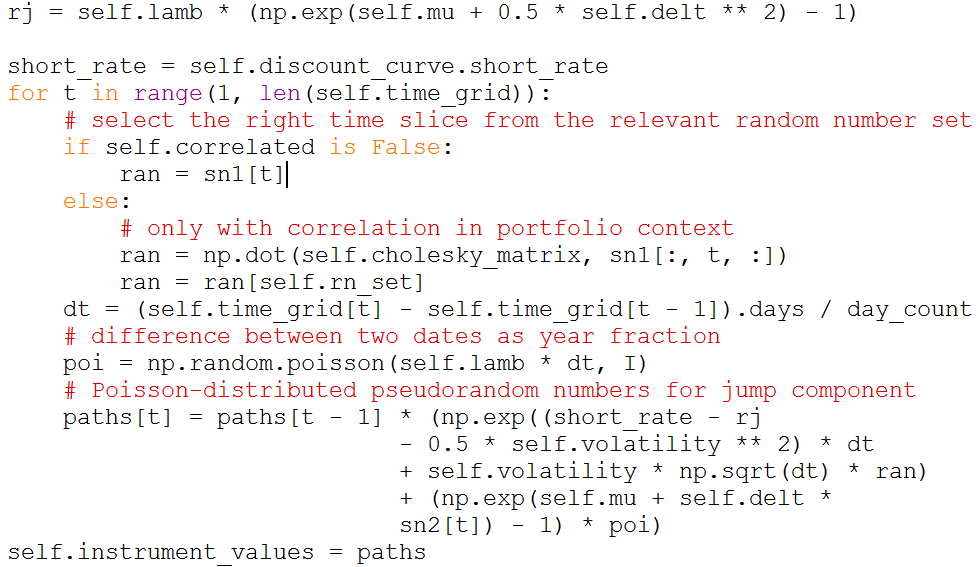
\includegraphics[scale=0.47]{jd_generate_path_2.png}
\end{figure}
\end{frame}

%------------------------------------------------
\begin{frame}
\frametitle{Jump Diffusion - Use Case}
\begin{figure}[H]
	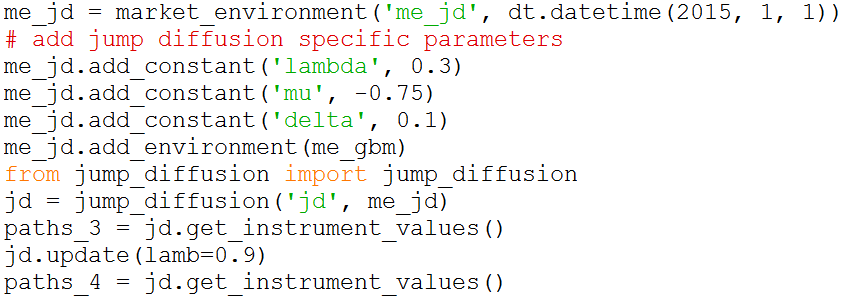
\includegraphics[scale=0.45]{jd_use_case.png}
\end{figure}
The Jump Diffusion simulation class is able to:
\begin{itemize}
	\item Import parameters from market environment class
	\item Generate datetime object time grid (inherited)
	\item Get instrument values based on parameters
\end{itemize}
\end{frame}

\subsection{Square-root Diffusion}
%------------------------------------------------
\begin{frame}
\frametitle{Square-root diffusion model}
\begin{center}
	$dx_{t} = \kappa(\theta-x_{t})dt + \sigma\sqrt{x_{t}}dZ_{t}$
\end{center}
\emph{Euler discretization}:
\begin{center}
	letting $s = t-^{\Delta}t$, and $x^{+} = max(x,0)$\\[3mm]
	$\tilde{x}_{t} = \tilde{x}_{s} + \kappa(\theta-\tilde{x}_{s}^{+}){^{\Delta}t} + \sigma\sqrt{\tilde{x}_{s}^{+}{^{\Delta}t}}z_{t}$\\[3mm]
	$x_{t} = \tilde{x}_{t}^{+}$
\end{center}
\end{frame}

%------------------------------------------------
\begin{frame}
\frametitle{Square-root Diffusion - implementation}
\begin{figure}[H]
	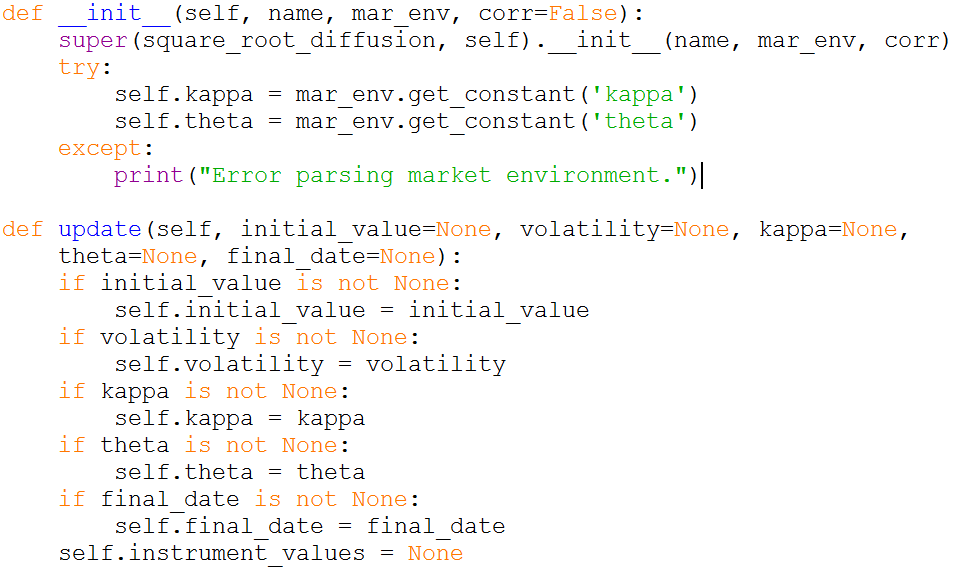
\includegraphics[scale=0.42]{srd_init_update.png}
\end{figure}
\end{frame}

%------------------------------------------------
\begin{frame}
\frametitle{Square-root Diffusion - implementation}
This part of generate\_path is repeated, maybe we can capture this feature
\begin{figure}[H]
	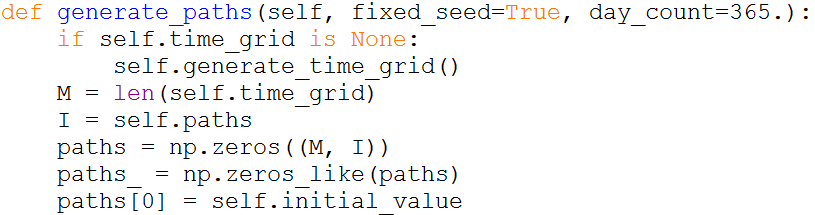
\includegraphics[scale=0.4]{srd_generate_path_1.png}
\end{figure}
\end{frame}

%------------------------------------------------
\begin{frame}
\frametitle{Square-root Diffusion - implementation}
\begin{figure}[H]
	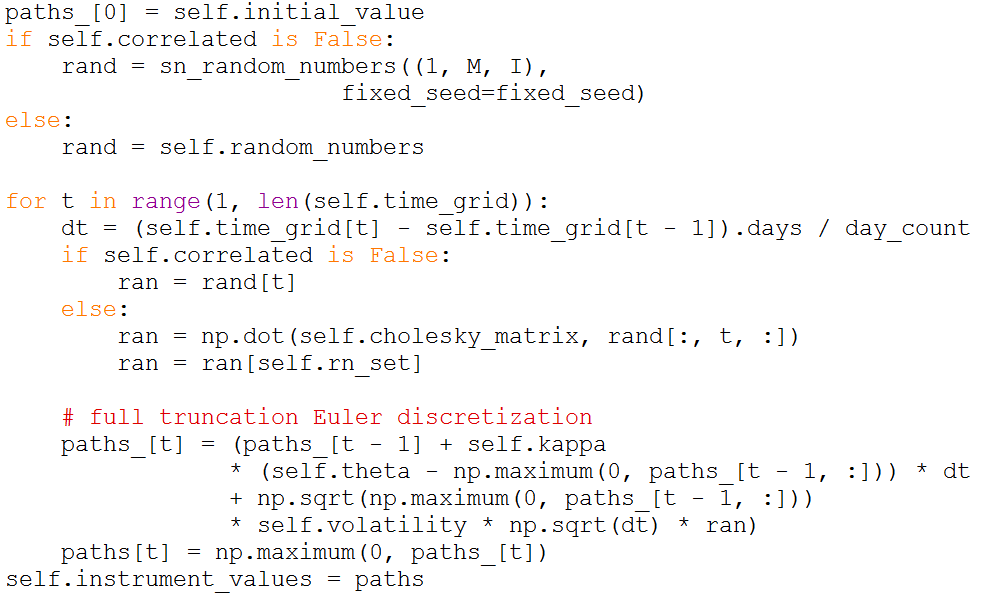
\includegraphics[scale=0.47]{srd_generate_path_2.png}
\end{figure}
\end{frame}

%------------------------------------------------
\begin{frame}
\frametitle{Square-root Diffusion - Use Case}
\begin{figure}[H]
	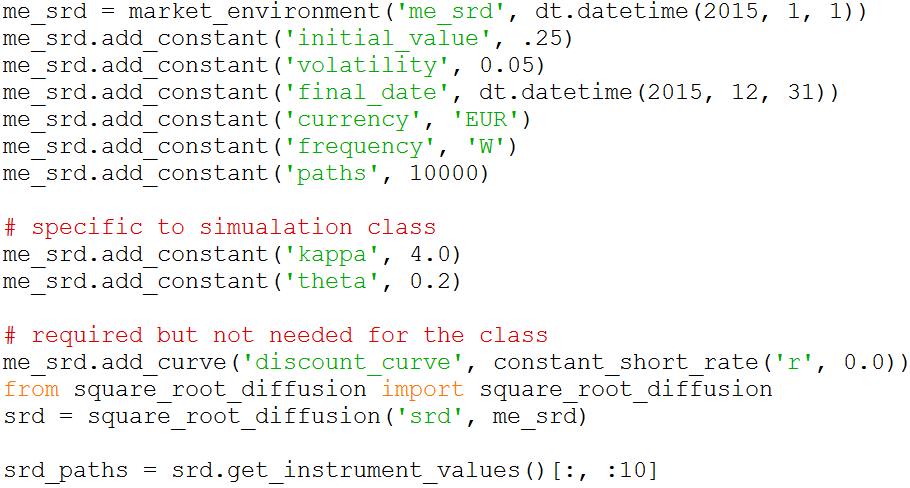
\includegraphics[scale=0.44]{srd_use_case.png}
\end{figure}
The Square-root Diffusion simulation class is able to:
\begin{itemize}
	\item Import parameters from market environment class
	\item Generate datetime object time grid (inherited)
	\item Get instrument values based on parameters
\end{itemize}
\end{frame}

\subsection{Capture common features}
%------------------------------------------------
\begin{frame}
\frametitle{Capture common features from generate\_path() method}
We now define a new method in the simulation class to be inherited.
\begin{figure}[H]
	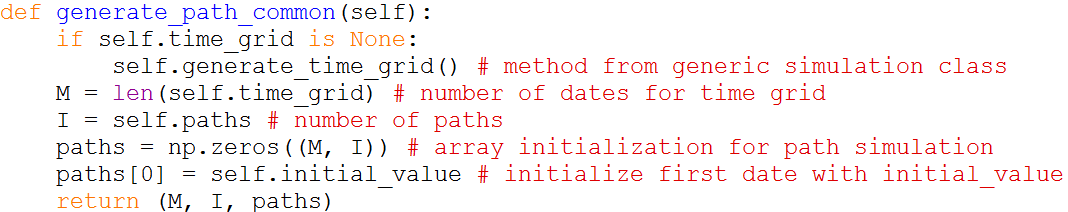
\includegraphics[scale=0.42]{generate_path_common.png}
\end{figure}
And it will then be called by the subclasses using this statement:
\begin{figure}[H]
	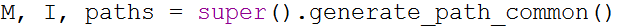
\includegraphics[scale=0.5]{call_super_generate_path_common.png}
\end{figure}
\end{frame}

\subsection{Wrapper class}

%------------------------------------------------
\begin{frame}
\frametitle{Wrapper class - implementation}
\begin{figure}[H]
	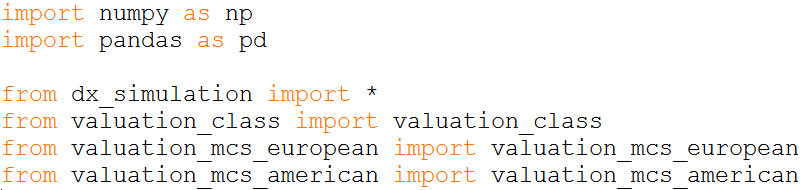
\includegraphics[scale=0.48]{wrapper_class.png}
\end{figure}
With this $dx\_frame.py$, we are now able to import the valuation framework package as well the simulation classes in one line.
\end{frame}

%------------------------------------------------
\begin{frame}
\frametitle{Wrapper class - testing}
Now we need to enhance the $\_\_init\_\_.py$ which initially has the same content as $dx\_frame.py$ in the same directory to include importing the simulation classes.
\begin{figure}[H]
	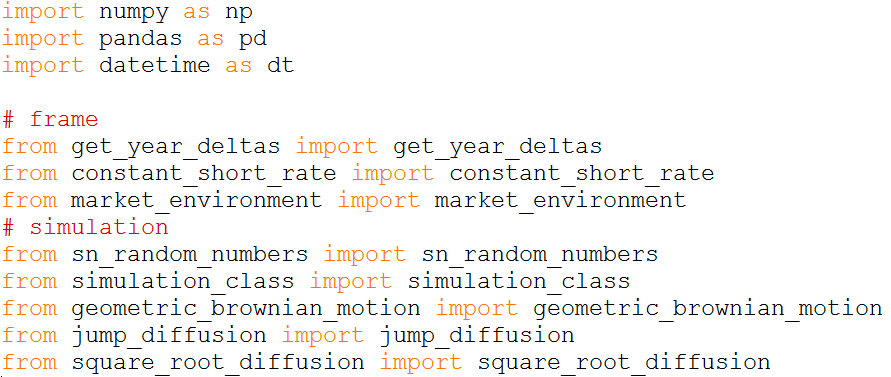
\includegraphics[scale=0.48]{import_wrapper_class.png}
\end{figure}
\end{frame}

%-----------------------------------------------
\begin{frame}
\Huge{\centerline{Thank You}}
\begin{center}
\begin{normalsize}
\emph{E0007424@u.nus.edu}
\end{normalsize}
\end{center}
\end{frame}

%------------------------------------------------

\end{document} 